\documentclass{warpdoc}
\newlength\lengthfigure                  % declare a figure width unit
\setlength\lengthfigure{0.158\textwidth} % make the figure width unit scale with the textwidth
\usepackage{psfrag}         % use it to substitute a string in a eps figure
\usepackage{subfigure}
\usepackage{rotating}
\usepackage{pstricks}
\usepackage[innercaption]{sidecap} % the cute space-saving side captions
\usepackage{scalefnt}
%\usepackage{amsbsy}

%%%%%%%%%%%%%=--NEW COMMANDS BEGINS--=%%%%%%%%%%%%%%%%%%%%%%%%%%%%%%%%%%
\newcommand{\rhos}{\rho} 
\newcommand{\Cv}{{C_{\rm v}}} 
\newcommand{\Cp}{{C_{\rm p}}} 
\newcommand{\nd}{{{n}_{\rm d}}}
\newcommand{\ns}{{{n}_{\rm s}}}
\newcommand{\nn}{{{n}_{\rm n}}}
\newcommand{\ndm}{{\bar{n}_{\rm d}}}
\newcommand{\nsm}{{\bar{n}_{\rm s}}}
\newcommand{\turb}{_{\rm T}}
\newcommand{\mut}{{\mu\turb}}
\newcommand{\mfa}{\scriptscriptstyle}
\newcommand{\mfb}{\scriptstyle}
\newcommand{\mfc}{\textstyle}
\newcommand{\mfd}{\displaystyle}
\newcommand{\hlinex}{\vspace{-0.34cm}~~\\ \hline \vspace{-0.31cm}~~\\}
\newcommand{\hlinextop}{\vspace{-0.46cm}~~\\ \hline \hline \vspace{-0.32cm}~~\\}
\newcommand{\hlinexbot}{\vspace{-0.37cm}~~\\ \hline \hline \vspace{-0.50cm}~~\\}
\newcommand{\tablespacing}{\vspace{-0.4cm}}
\newcommand{\fontxfig}{\footnotesize\scalefont{0.918}}
\newcommand{\fontgnu}{\footnotesize\scalefont{0.896}}
\renewcommand{\fontsizetable}{\footnotesize\scalefont{1.0}}
\renewcommand{\fontsizefigure}{\footnotesize}
\renewcommand{\vec}[1]{\pmb{#1}}
\setcounter{tocdepth}{3}
\let\citen\cite

%%%%%%%%%%%%%=--NEW COMMANDS BEGINS--=%%%%%%%%%%%%%%%%%%%%%%%%%%%%%%%%%%

\setcounter{tocdepth}{3}

%%%%%%%%%%%%%=--NEW COMMANDS ENDS--=%%%%%%%%%%%%%%%%%%%%%%%%%%%%%%%%%%%%



\author{
  Bernard Parent
}

\email{
  bernparent@gmail.com
}

\department{
  Department of Aerospace and Mechanical Engineering	
}

\institution{
  University of Arizona
}

\title{
  GRIDG: a Library of Subroutines for Generating Structured Grids 
}

\date{
  1999 -- Revised in 2016, 2018
}

%\setlength\nomenclaturelabelwidth{0.13\hsize}  % optional, default is 0.03\hsize
%\setlength\nomenclaturecolumnsep{0.09\hsize}  % optional, default is 0.06\hsize

\nomenclature{

  \begin{nomenclaturelist}{Roman symbols}
   \item[$a$] speed of sound
  \end{nomenclaturelist}
}


\abstract{
abstract
}

\begin{document}
  \pagestyle{headings}
  \pagenumbering{arabic}
  \setcounter{page}{1}
%%  \maketitle
  \makewarpdoctitle
%  \makeabstract
  \tableofcontents
%  \makenomenclature
%%  \listoftables
%%  \listoffigures




\sloppy

\section{List of GRIDG Actions}

This section outlines all the
actions within the GRIDG library. It is noted
that since the GRIDG library uses the SOAP interpreter library, all
builtin functions, actions, loops, if conditions, constants, etc.
part of the SOAP interpreter language are also available here.

\subsection{\emph{Size}}

Before creating the grid, a size must be specified.
Consequently, this must be the first action to be performed.
The following would allocate enough RAM to store a $10\times 20$
mesh:
%
\begin{verbatim}
  Size( 1,1,  10,20 );
\end{verbatim}
%
with $i$ ranging from 1 to 10 and $j$ ranging from 1 to 20. Similarly,
a $10 \times 10 \times 10$ 3D mesh can be created as:
%
\begin{verbatim}
  Size( 1,1,1,  10,10,10 );
\end{verbatim}
%

\subsection{\emph{Point}}

\verb|Point| fixes $x,~y,~z$ at one grid node only.
For example,
%
\begin{verbatim}
  Point( 5,7,   0.1,0.3 );
\end{verbatim}
%
would set the grid node $\left( i=5,~j=7 \right)$ to $\left( x=0.1,~y=0.3\right)$,

\subsection{\emph{Corners}}

The \verb|Corners| command is simply a short-hand notation
for fixing the $x,y,z$ values of the 8 nodes in 3D and 4 nodes
in 2D at the corners of a box
by specifying only the bottom-left-near and top-right-far corner nodes.
For example,
%
\begin{verbatim}
  Corners( i1,j1,k1,  i2,j2,k2,  
           x1,y1,z1,  x2,y2,z2 );
\end{verbatim}
%
is equivalent to:
%
\begin{verbatim}
  Point( i1,j1,k1, x1,y1,z1 );  Point( i2,j1,k1, x2,y1,z1 );
  Point( i1,j2,k1, x1,y2,z1 );  Point( i2,j2,k1, x2,y2,z1 );
  Point( i1,j1,k2, x1,y1,z2 );  Point( i2,j1,k2, x2,y1,z2 );
  Point( i1,j2,k2, x1,y2,z2 );  Point( i2,j2,k2, x2,y2,z2 );
\end{verbatim}
%
but much shorter. In a two-dimensional grid,
%
\begin{verbatim}
  Corners( i1,j1, i2,j2,  x1,y1, x2,y2 );
\end{verbatim}
%
would correspond to:
%
\begin{verbatim}
  Point( i1,j1, x1,y1 );  Point( i2,j1, x2,y1 );
  Point( i1,j2, x1,y2 );  Point( i2,j2, x2,y2 );
\end{verbatim}
%

\subsection{\emph{JoinCorners}}

A \emph{JoinCorners} action is applied to a
subregion of the grid 
ranging from \verb|i1,j1,k1| to \verb|i2,j2,k2|. Before applying
the block command, one must ensure that the $x,y,z$ values of each corner
of the rectangular subregion is specified: i.e. \verb|i1,j1,k1|,
\verb|i2,j1,k1|, \verb|i1,j2,k1|, etc. These values will
be read and joined with line segments to form the edges of
the subregion. The edges are thereafter joined with line segments 
to form planes, which are themselves joined with line segments to complete
the gridding of the subregion.

It is noted that the \verb|JoinCorners|
action is such that all segments part of the block \emph{consist
of straight lines only}. The node spacing along each segment
is not necessarily constant however, the segment's clustering
being specified at call time for all $i$s, $j$s and $k$s:
%
\begin{verbatim}
  JoinCorners(i1,j1,k1, i2,j2,k2,
       EE,0.5,1.0,1.0, {<- clustering for segments along i}
       EE,0.5,1.0,1.0, {<- clustering '   '        '     j}
       EE,0.5,1.0,1.0  {<- clustering '   '        '     k}
  );
\end{verbatim}
%
which would create an equispaced mesh along $i,~j,~k$. 

It can be seen that 4 arguments are
necessary to specify the segment's clustering. The first argument
(i.e. EE in the latter example) is made up of two letters
each specifying which type of clustering
occurs in the lower and upper portions of the segment respectively.
Three types of clustering are available: 
\begin{enumerate}
\item
 'E': Exponential clustering.
  This will result in a node spacing with a user-specified exponential growth. 
\item 'F': Fixed spacing at segment's start or end. Should 'F' be specified for
the lower or upper parts of the segment, the spacing would obviously
be fixed at the lower or upper end of such segment; 
\item 'G': Grabbed spacing. Similar to 'F' but the spacing at the start/end of the segment
  is ``grabbed'' from the mesh instead of being user-specified. Obviously, for grabbed
spacing to work properly, one must make sure there is a spacing to be
grabbed either at the segment's end or start. 
\end{enumerate}
Further, a special type of segment
clustering (referred to herein as ``weak clustering'')
where a certain fraction of the nodes of the segment are
equally spaced and the clustering takes place on the rest. This can be specified by 
 'ff', 'fg', 'gf' or 'gg',
where the letters 'f' and 'g' perform similarly as their uppercase
counterparts. 

The second argument denotes the fraction of the segment's nodes
to be placed in the lower portion of the segment. For example,
should the second argument be $0.7$ then 70\% of the nodes of the segment
will be placed in the lower section of the segment. When using weak
clustering, the second argument refers to the portion of the nodes
that are equally spaced within the segment.

The third and fourth arguments are used in conjunction with the spacing
type. For example, should the first argument read 'EF', then the user
is expected to specify the exponential growth of the lower part
of the segment as the third argument, while specifying the fixed spacing
at the segment's end as the fourth argument. The following segment
clustering
%
\begin{verbatim}
   EF,0.8,1.0,0.01
\end{verbatim}
%
hence specifies that 80\% of the nodes are to be placed
in the lower part of the segment which is to be equally spaced
(exponential growth of 1.0), while the rest of the nodes in
the upper segment have such an exponential growth that the last
node spacing is 0.01 units. For a second example, let us consider
a cluster involving grabbing:
%
\begin{verbatim}
   FG,0.5,0.001,0
\end{verbatim}
%
which allocates equal number of nodes to both the upper and lower
parts, fixes the first node's spacing to 0.001 units, grabs the last
node's spacing from the grid and calculates the growth
in both parts of the segment to obtain such spacings at both ends.
Note that the fourth argument's value has no effect on the segment's
construction since the nodes spacing is grabbed from the grid, and not specified
by the user.

Segments can be specified within several actions, such as the  \verb|JoinCorners| action for instance:
%
\begin{verbatim}
  JoinCorners(i1,j1,k1, i2,j2,k2,
       EE, 0.5, 1.0, 1.0,
       GE, 0.5, 0,   1.0,
       EE, 0.5, 1.0, 1.0
  );
\end{verbatim}
%
The latter creates equally spaced segments along $i$ and $k$;
along $j$, the upper part of the segments would be equispaced,
while the lower part would exhibit such exponential growth to
match the grid spacing at j1.


\subsection{\emph{Join}}

As its name implies, \verb|Join| joins two regions
of the grid together using a syntax similar to the
\verb|JoinCorners| action. Both regions must already
have been gridded obviously. Its syntax in 3D is as follows:
%
\begin{verbatim}
  Join(i1,j1,k1, i2,j2,k2, i,
       EE, 0.5e0, 1.0e0, 1.0e0
  );
\end{verbatim}
%
The latter creates a grid located in the subregion
(\verb|i1|$\leq$\verb|i|$\leq$\verb|i2|,
  \verb|j1|$\leq$\verb|j|$\leq$\verb|j2|,
  \verb|k1|$\leq$\verb|k|$\leq$\verb|k2|)
by joining the planes \verb|i|$=$\verb|i1| and \verb|i|$=$\verb|i2| with
one-dimensional segments of similar form as the ones used in the
\verb|JoinCorners| command. The direction of the joint is
specified in the seventh parameter as being here along i
(but could also be along j or k if so desired). Note that
in this particular example, the $x,y,z$ values on the planes
\verb|i|=\verb|i1| and \verb|i|=\verb|i2| must have determined prior
to applying the joint.  The second line of the \verb|Join|
action, i.e. ``\verb|EE, 0.5e0, 1.0e0, 1.0e0|'', specifies the clustering
along the joint direction which follows the same syntax as
the clustering specified within the \verb|JoinCorners| command.

When used on a 2D grid, \verb|Join| is to be used as follows:
%
\begin{verbatim}
  Join(i1,j1, i2,j2, i,
       EE, 0.5e0, 1.0e0, 1.0e0
  );
\end{verbatim}



\subsection{\emph{JoinFaces}}

\verb|JoinFaces| joins all nodes on the outside shell (or perimeter in 2D) of the
grid region (\verb|i1|$\leq$\verb|i|$\leq$\verb|i2|,
  \verb|j1|$\leq$\verb|j|$\leq$\verb|j2|,
  \verb|k1|$\leq$\verb|k|$\leq$\verb|k2|). In 3D the syntax takes on the form:
%
\begin{verbatim}
  JoinFaces(i1,j1,k1, i2,j2,k2);
\end{verbatim}
%
while in 2D, one would write:
%
\begin{verbatim}
  JoinFaces(i1,j1, i2,j2);
\end{verbatim}
%
Of course, the node positions must already have been given a value prior
to the call to the \verb|JoinFaces| command on
\verb|i=i1|, \verb|i=i2|, \verb|j=j1|, \verb|j=j2|, \verb|k=k1| and
\verb|k=k2|. The algorithm was implemented by Dr.\ Derrick Alexander.


\subsection{\emph{Plane}}

\verb|Plane| creates a plane inside the
grid region (\verb|i1|$\leq$\verb|i|$\leq$\verb|i2|,
  \verb|j1|$\leq$\verb|j|$\leq$\verb|j2|,
  \verb|k1|$\leq$\verb|k|$\leq$\verb|k2|) where either
  \verb|j1=j2| or \verb|i1=i2| or \verb|k1=k2|. Its syntax in 3D is as follows:
%
\begin{verbatim}
  Plane(i1,j1,k1, i2,j2,k2);
\end{verbatim}
%
It is noted that the plane generation algorithm  assumes that a plane
with a tangent vector pointing more or less along $x$ lies on \verb|i=i1=i2|, but
should the tangent vector point along $y$ it is assumed that \verb|j=j1=j2|
and similarly for the third dimension.
The algorithm can be used in 3D only and is termed \verb|Plane|. 
The node positions on the plane perimeter must already have been given a value prior
to the call to the \verb|Plane| command. The algorithm was 
implemented by Dr.\ Derrick Alexander.


\subsection{\emph{Rotate}}

After all points in a subregion have been assigned
a  $x,y,z$ value, they can be rotated around a pivot
using the \verb|Rotate| command:
%
\begin{verbatim}
  Rotate(i1,j1,k1, i2,j2,k2,
         pivot_x,pivot_y,pivot_z,
         theta,x);
\end{verbatim}
%
which would rotate all nodes in the region
(\verb|i1|$\leq$\verb|i|$\leq$\verb|i2|,
  \verb|j1|$\leq$\verb|j|$\leq$\verb|j2|,
  \verb|k1|$\leq$\verb|k|$\leq$\verb|k2|)
around the pivot point located at $x=$\verb|pivot_x|,
$y=$\verb|pivot_y| and $z=$\verb|pivot_z| by the angle
\verb|theta| in radians. The rotation will be performed with respect to
the \verb|x| axis in this case, and the sign of
the rotation angle follows the ``right-hand''
convention. Of course, \verb|x| can be replaced by
\verb|y| or \verb|z|.

In 2 dimensions, the axis of rotation does not need to be specified
as it is perpendicular to the 2D plane:
%
\begin{verbatim}
  Rotate(i1,j1, i2,j2,
         pivot_x,pivot_y, theta);
\end{verbatim}
%



\subsection{\emph{Translate}}

A translation of a subregion defined by
(\verb|i1|$\leq$\verb|i|$\leq$\verb|i2|,
  \verb|j1|$\leq$\verb|j|$\leq$\verb|j2|,
  \verb|k1|$\leq$\verb|k|$\leq$\verb|k2|)
by the vector (\verb|delta_x|, \verb|delta_y|, \verb|delta_z|)
can be accomplished through:
%
\begin{verbatim}
  Translate(i1,j1,k1, i2,j2,k2,
            delta_x,delta_y,delta_z);
\end{verbatim}
%
The latter  translates all points contained in such subregion by
 \verb|delta_x| units along $x$, \verb|delta_y| units along $y$, etc.
The 2D form of the latter is straightforward:
%
\begin{verbatim}
  Translate(i1,j1, i2,j2,
            delta_x,delta_y);
\end{verbatim}
%


\subsection{\emph{Copy}}

It is possible to copy the $x, y, z$ coordinates of all nodes
of a subregion delimited by
(\verb|i1|$\leq$\verb|i|$\leq$\verb|i2|,
  \verb|j1|$\leq$\verb|j|$\leq$\verb|j2|,
  \verb|k1|$\leq$\verb|k|$\leq$\verb|k2|)
to another subregion of the same size but starting
at (\verb|id,jd,kd|) instead of (\verb|i1,j1,k1|) through the use
of the copy command:
%
\begin{verbatim}
  Copy(i1,j1,k1, i2,j2,k2,
       id,jd,kd);
\end{verbatim}
%
while the 2D equivalent takes the form:
%
\begin{verbatim}
  Copy(i1,j1, i2,j2,
       id,jd);
\end{verbatim}
%


\subsection{\emph{Equation}}

The \verb|Equation| action permits the specification
of a $x$-$y$-$z$-dependent equation defining a certain
surface or curve. It is noted that
when using this action on a subregion delimited by
(\verb|i1|$\leq$\verb|i|$\leq$\verb|i2|,
  \verb|j1|$\leq$\verb|j|$\leq$\verb|j2|,
  \verb|k1|$\leq$\verb|k|$\leq$\verb|k2|),
it must be made sure that all points in this subregion have already been
assigned a $x, y, z$ value from which a new $x$, or a new $y$ or a
new $z$ can be determined with the aid of the equation.
For example, consider the following:
%
\begin{verbatim}
  Equation(
    i1,j1,k1, i2,j2,k2,
    z,   { variable (x,y or z) to change in the subregion }
    z=y+x^2+x^3+x^0.15+sin(10*x) { the equation }
  );
\end{verbatim}
%
Within the Equation() command, the first line specifies the subregion affected, 
while the second line  specificies  the variable to be
changed in this subregion (i.e.\ here  \verb|z|, leaving \verb|x| and \verb|y|
unaffected), and the third line specifies the equation defining \verb|z|. A Newton-Raphson 
iteration is used to find the closest root with the initial conditions grabbed
from the grid. Here is another example of the Equation() command, this time involving
a non-linear equation:
%
\begin{verbatim}
  Equation(
    i1,j1,k1, i2,j2,k2,
    z,   { variable (x,y or z) to change in the subregion }
    (z^4+z^2+z^0.2)=y+x^2+x^3+x^0.15+sin(10*x) { the equation }
  );
\end{verbatim}
%
Should the equation specified not be linear, one must be 
careful to specify ``good'' initial conditions so that the root solver converges to the desired
root. 

Lastly, a 2D example:
%
\begin{verbatim}
  Equation(
    i1,j1, i2,j2,
    x,    { variable (x or y) to change in the subregion }
    x=y^3 { the equation }
  );
\end{verbatim}
%


\subsection{\emph{Spline}}

The \verb|Spline| action permits the modification of the $x$, $y$, $z$ coordinates
through a cubic spline curve. 
When using this action on a subregion delimited by
(\verb|i1|$\leq$\verb|i|$\leq$\verb|i2|,
  \verb|j1|$\leq$\verb|j|$\leq$\verb|j2|,
  \verb|k1|$\leq$\verb|k|$\leq$\verb|k2|),
it must be made sure that all points in this subregion have already been
assigned a $x, y, z$ value from which a new $x$, or a new $y$ or a
new $z$ can be determined with the aid of the spline.
For example, consider the following:
%
\begin{verbatim}
  Spline(
    i1,j1,k1, i2,j2,k2, {subregion affected}
    y(x),   {changes y as a function of x}
    x1,y1, x2,y2, x3,y3  {data points constructing spline}
  );
\end{verbatim}
%
The first line specifies the subregion affected. 
The second line  specifies  which coordinate to change in this subregion as well as the coordinate on which the spline depends. Thus, specifying \verb|y(x)| leads to the spline yielding $y$ as a function of $x$, and to the $y$ coordinate being altered according to the spline in the subregion while the $x$ and $z$ coordinates are unaltered. 
The third line consists of the data points that are used to construct the spline.

Here is another example of the Spline() command, this time involving
$x$ being varied as a function of $z$:
%
\begin{verbatim}
  Spline(
    i1,j1,k1, i2,j2,k2,
    x(z),   {changes x as a function of z}
    z1,x1, z2,x2, z3,x3, z4,x4, z5,x5  
  );
\end{verbatim}
%
Note that the data points must be such that they ``follow'' one another. Thus in the first example given above the data points must be such that \verb|x3>x2>x1|, and in the second example given, the data points must be such that \verb|z5>z4>z3>z2>z1|.

Lastly, a 2D example:
%
\begin{verbatim}
  Spline(
    i1,j1, i2,j2,
    x(y),   {changes x as a function of y}
    y1,x1, y2,x2, y3,x3, y4,x4  
  );
\end{verbatim}
%



\subsection{\emph{Mirror}}

After all points in a subregion have been assigned
a  $x,y,z$ value, they can be mirrored with respect to a plane using the \verb|Mirror| command. For instance,
%
\begin{verbatim}
  Mirror(i1,j1,k1, i2,j2,k2, x, 0.2);
\end{verbatim}
%
mirrors all nodes in the region
(\verb|i1|$\leq$\verb|i|$\leq$\verb|i2|,
  \verb|j1|$\leq$\verb|j|$\leq$\verb|j2|,
  \verb|k1|$\leq$\verb|k|$\leq$\verb|k2|)
with respect to the plane  $x=0.2$.
In 2 dimensions, the command can be called in this fashion
%
\begin{verbatim}
  Mirror(i1,j1, i2,j2, y, 0.3);
\end{verbatim}
%


\subsection{\emph{Scale}}

A grid subregion can be scaled with respect to
an origin using the \verb|Scale| command. For instance,
%
\begin{verbatim}
  Scale(i1,j1,k1, i2,j2,k2,
        origin_x,origin_y,origin_z,
        scale_factor_x, scale_factor_y, scale_factor_z);
\end{verbatim}
%
 scales the region
(\verb|i1|$\leq$\verb|i|$\leq$\verb|i2|,
  \verb|j1|$\leq$\verb|j|$\leq$\verb|j2|,
  \verb|k1|$\leq$\verb|k|$\leq$\verb|k2|)
with respect to the origin located at $x=$\verb|origin_x|,
$y=$\verb|origin_y| and $z=$\verb|origin_z| by the factor
\verb|scale_factor_x| along $x$ and by the factor
\verb|scale_factor_y| along $y$, and by the factor
\verb|scale_factor_z| along $z$.

In 2 dimensions, the Scale command can be called as follows:
%
\begin{verbatim}
  Scale(i1,j1, i2,j2,
        origin_x,origin_y, scale_factor_x, scale_factor_y);
\end{verbatim}
%



\subsection{\emph{ReverseIndex}}

The index ($i$, $j$ or $k$) of all points in a subregion
can be reversed with the
\verb|ReverseIndex| command. For instance,
%
\begin{verbatim}
  ReverseIndex(4,4,4, 10,10,10, i);
\end{verbatim}
%
 reverses the $i$ index in the region
(\verb|4|$\leq$\verb|i|$\leq$\verb|10|,
  \verb|4|$\leq$\verb|j|$\leq$\verb|10|,
  \verb|4|$\leq$\verb|k|$\leq$\verb|10|).
Hence in this case, the $x$, $y$, $z$ values of
point $i,j,k$ would be interchanged with the values
at point $10-(i-4),j,k$ for all $i,j,k$ in the subregion.

In 2 dimensions, the action can be called as
%
\begin{verbatim}
  ReverseIndex(i1,j1, i2,j2, i);
\end{verbatim}
%









\section{List of GRIDG Functions}

This section outlines all the functions within the GRIDG library. 

\subsection{\emph{\_x()~,...}}

The $x$, $y$ and $z$ values of any node can be accessed
anywhere by using the \verb|_x(i,j,k)|, \verb|_y(i,j,k)|
and \verb|_z(i,j,k)| functions respectively. The latter can
also be used  as part of an argument passed to any action outlined
above. For example, the following would output the values
of $x$ to the screen for the nodes ranging from (\verb|i1,0,0|)
to (\verb|i2,0,0|):
%
\begin{verbatim}
  for ( i, i1, i2,
    writeln(_x(i,0,0));
  );
\end{verbatim}
%
In 2D, only two arguments are passed of course, i.e. \verb|i|
and \verb|j|.



\section{Examples of Meshes Generated with GRIDG}


\subsection{2D Quadrilateral}


%
\begin{figure}[h]
\vspace{0.3cm}
   \fontxfig
   \psfrag{X}[][][1][0]{$x$ [m]}
   \psfrag{Y}[][][1][0]{$y$ [m]}
   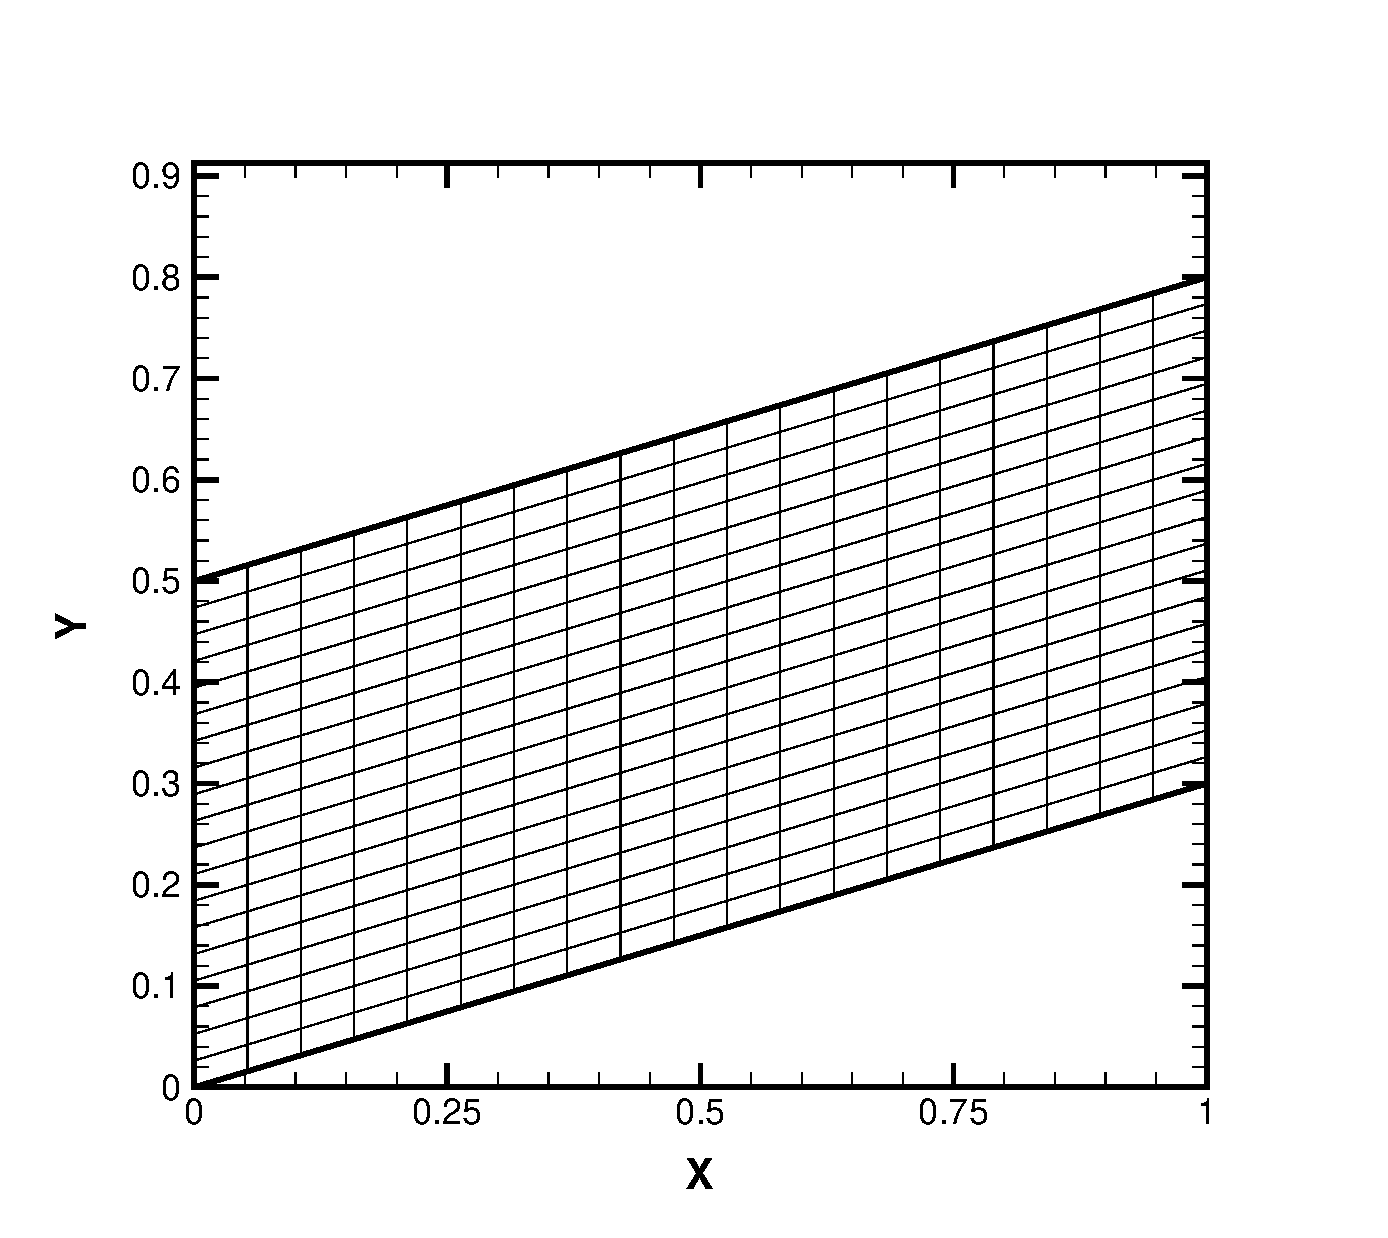
\includegraphics[width=3.0in]{grid.2D.quad.eps}
\caption{2D quadrilateral grid output}
\label{fig:gridquad}
\end{figure}
%

Probably the easiest grid to generate, and hence a good starting point
is an equally spaced quadrilateral.
The following grid algorithm will result in the 2D quadrilateral
shown in figure \ref{fig:gridquad}:
%
\begin{verbatim}
  01  is=1;  js=1;
  02  ie=20; je=20;
  03
  04  Grid(
  05    Size ( is,js, ie,je );
  06    Point( is,js, 0,0 );    Point( ie,js, 1,0.3 );
  07    Point( is,je, 0,0.5 );  Point( ie,je, 1,0.8 );
  08    JoinCorners( is,js, ie,je,
  09           EE,0.5, 1,1,   EE,0.5, 1,1 );
  10  );
\end{verbatim}
%
where lines 6-7 fix the $x$ and $y$ values of the corners of
the mesh and line 8 fills out the quadrilateral with
equally spaced straight lines.



\subsection{2D Wedge}

%
\begin{figure}[h]
\vspace{0.3cm}
   \fontxfig
   \psfrag{X}[][][1][0]{$x$ [m]}
   \psfrag{Y}[][][1][0]{$y$ [m]}
   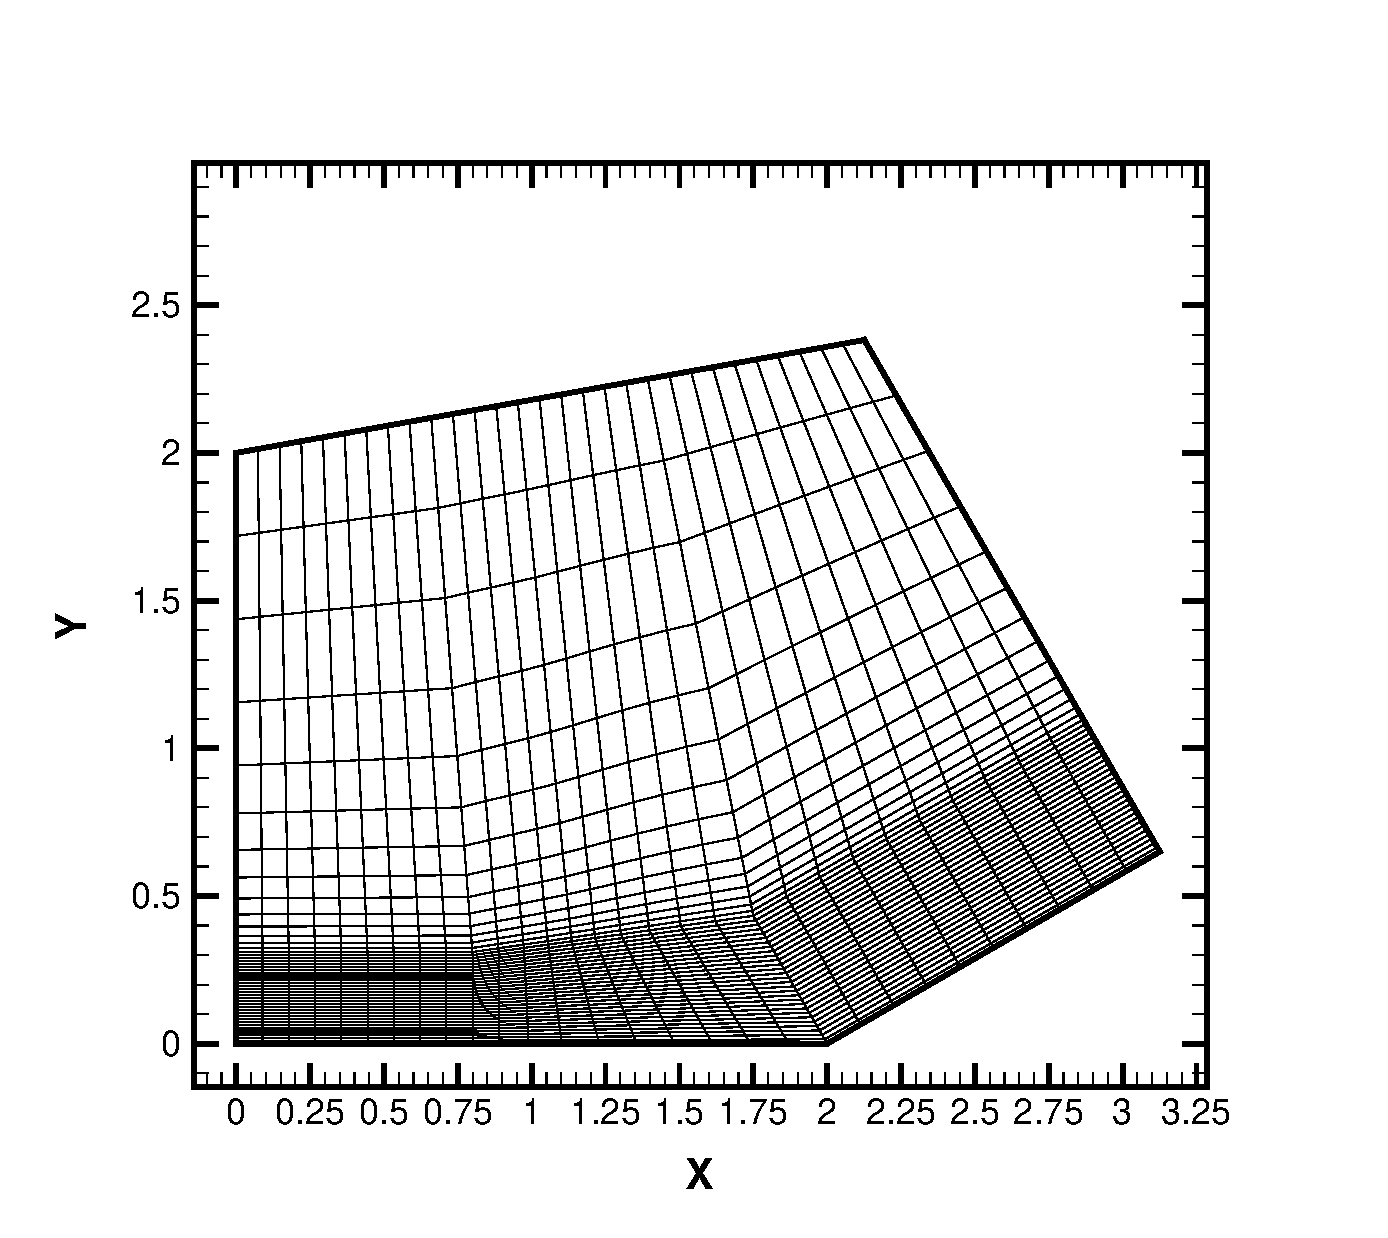
\includegraphics[width=3.0in]{grid.2D.wedge.eps}
\caption{2D wedge mesh.}
\label{fig:gridwedge}
\end{figure}
%
The gridding of a flow interacting with a wedge with clustering at the surfaces is shown in figure \ref{fig:gridwedge}. The code used
to create this figure is the following (minus the line numbering):
%
\begin{verbatim}
  01  i1=1; i2=10; i3=20; i4=30;
  02  j1=1; j2=30; j3=45;
  03  angle=rad(30); {30 degrees angle}
  04  bh1=0.3;       {boundary layer height before wedge}
  05  bh2=0.5;       {boundary layer height after wedge}
  06  l1=0.8;        {length of plate before wedge}
  07  l2=1.3;        {length of plate after wedge}
  08  x=2;           {wedge start}
  09  h1=2;          {height of domain}
  10
  11  Grid(
  12    Size        ( i1,j1, i4,j3 );
  13    Corners     ( i1,j1, i2,j2, 0,0, l1,bh1);
  14    JoinCorners ( i1,j1, i2,j2, EE,0.5,1,1, EE,0.5,1,1 );
  15    Corners     ( i3,j1, i4,j2, 0,0, l2,bh2);
  16    JoinCorners ( i3,j1, i4,j2, EE,0.5,1,1, EE,0.5,1,1 );
  17    Rotate      ( i3,j1, i4,j2, 0,0, angle);
  18    Translate   ( i3,j1, i4,j2, x,0 );
  19    Join        ( i2,j1, i3,j2, i, GG,0.5,0,0 );
  20    Point       ( i1,j3, 0,h1);
  21    Point       ( i4,j3, x+l2,h1);
  22    Rotate      ( i4,j3, i4,j3, x,0, angle);
  23    JoinCorners ( i1,j3, i4,j3, EE,0.5,1,1, NO,0.5,1,1 );
  24    Join        ( i1,j2, i4,j3, j, GE,0.9,1,1 );
  25  );
\end{verbatim}
%
Note that
the clustered zone (near the bottom boundary) is made up of
two equispaced zones (lines 13-18) joined together on line 19.
Once the clustered zone is gridded, a one dimensional segment
is created at \verb|j=j3| (lines 20-23) which is joined to the
clustered region on line 24.


\subsection{2D Wavy Wall}

%
\begin{figure}[h]
\vspace{0.3cm}
   \fontxfig
   \psfrag{X}[][][1][0]{$x$ [m]}
   \psfrag{Y}[][][1][0]{$y$ [m]}
   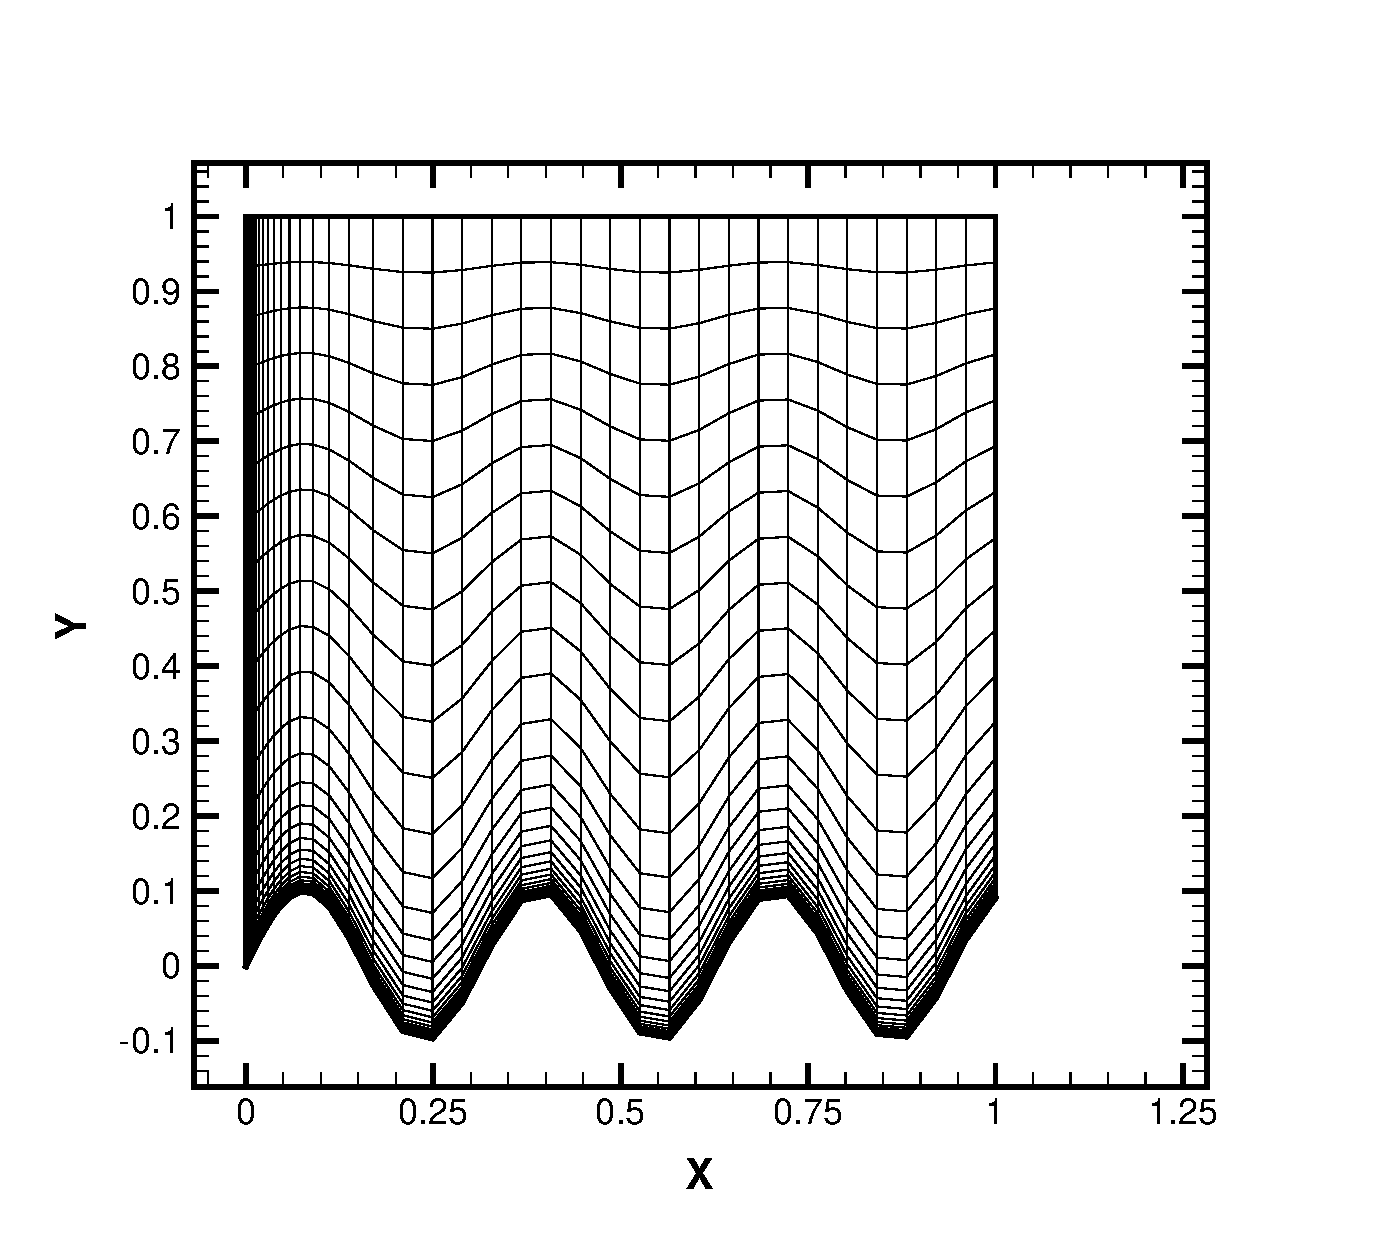
\includegraphics[width=3.0in]{grid.2D.sine.eps}
\caption{2D wavy wall mesh.}
\label{fig:gridsine}
\end{figure}
%
The ``wavy-wall'' mesh shown in Figure \ref{fig:gridsine} was created with
the following code:
%
\begin{verbatim}
  01  i1=1; i2=40;
  02  j1=1; j2=30;
  03  dwall=0.001;
  04
  05  Grid(
  06    Size        ( i1,j1, i2,j2 );
  07    Corners     ( i1,j1, i2,j2, 0,0, 1,1);
  08    JoinCorners ( i1,j1, i2,j1, FE,0.5,dwall,1, NO,0.5,1,1 );
  09    JoinCorners ( i1,j2, i2,j2, FE,0.5,dwall,1, NO,0.5,1,1 );
  10    Equation    ( i1,j1, i2,j1, y, y=0.1*sin(x*20));
  11    Join        ( i1,j1, i2,j2, j, FE,0.7,dwall,1 );
  12  );
\end{verbatim}
%
Line 7 fixes $x$ and $y$ at the four corners. Lines 8 and 9 create
one dimensional segments on the lower and upper boundaries respectively.
Line 10 changes $y$ along the 1D segment created on line 8 according
to the specified equation, while line 11 joins the lower segment
and the upper one.




\section{Implementation Details of the GRIDG One Dimensional Segments}


%
\begin{figure}[!b]
\vspace{0.3cm}
\center
   \fontxfig
   \psfrag{Lz}[][][1][0]{$L_{\zeta}$}
   \psfrag{i=1}[][][1][0]{$i=1$}
   \psfrag{i}[][][1][0]{$i$}
   \psfrag{i+1}[][][1][0]{$i+1$}
  \psfrag{i+2}[][][1][0]{$i+2$}
  \psfrag{i=N}[][][1][0]{$i=N$}
   \psfrag{Dzi}[][][1][0]{$\Delta \zeta_i$}
   \psfrag{Dzi1}[][][1][0]{$\Delta \zeta_{i+1}$}
  \psfrag{zeta}[l][l][1][0]{$\zeta$}
   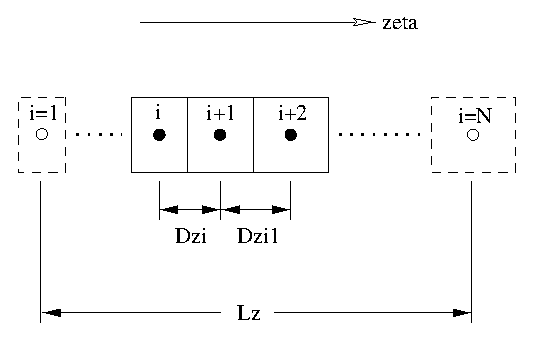
\includegraphics[width=2.83in]{meshspacing.eps}
\caption{Example of a non-equidistant mesh along the coordinate $\zeta$}
\label{fig:meshspacing}
\end{figure}
%

Some GRIDG commands documented in the previous section (i.e. \verb|JoinCorners|,
\verb|Join|) were constructed
using one-dimensional segments subroutines which are here outlined.
Referring to figure \ref{fig:meshspacing}, the mesh spacing
growth is defined by the Greek letter $\varepsilon$ and corresponds to:
%
\begin{equation}
\varepsilon=\frac{\Delta \zeta_{i+1} }{\Delta \zeta_{i}}
\label{eqn:spacing-growth}
\end{equation}
%
where $\zeta$ refers to a length coordinate.
It can be shown that a relation between $\varepsilon$, the number of
grid points $N$ and the length $L_{\zeta}$ (see figure \ref{fig:meshspacing})
corresponds to:
%
\begin{equation}
 L_{\zeta}=\sum_{i=1}^{N-1} \Delta \zeta_i
          =\sum_{i=1}^{N-1} \Delta \zeta_1 \varepsilon^{i-1}
          =\sum_{i=1}^{N-1} \frac{\Delta \zeta_{N-1}}{\varepsilon^{N-2}}\varepsilon^{i-1}
          =\sum_{i=1}^{N-1} {\Delta \zeta_{N-1}}\varepsilon^{i-N+1}
\label{eqn:spacing-growth-length}
\end{equation}
%
Hence, the gridding along $\zeta$ is fully determined provided
that three of the following constants are specified: $\varepsilon$, $L_\zeta$,
$\Delta \zeta_1$ or $\Delta \zeta_{N-1}$.






\subsection{Segment Type 1}

In this case, the two exponential node growth factors
$\varepsilon_L$ and $\varepsilon_H$ are specified,
with the only unknown being the first node distance
$\Delta \zeta_1$. Thus, the length of the lower segment section can be found from:
%
\begin{equation}
L_L=\mfd\sum_{i=1}^{N_L-1} \Delta \zeta_1 \varepsilon_L^{i-1} 
\end{equation}
%
and the length of the upper segment section  from:
%
\begin{equation}
 L_H=\mfd\sum_{i=1}^{N_H-1} \left( \Delta \zeta_1 \varepsilon_L^{N_L-2}  \right) \varepsilon_H^{i-1} 
\end{equation}
%
But the sum of the lengths of both sections must be equal to the total segment length:
%
\begin{equation}
L_H=L-L_L 
\end{equation}
%
Should the number of nodes be equal in both sections, we can say:
%
\begin{equation}
N_L=N/2 
\end{equation}
%
and
%
\begin{equation}
N_H=N-N_L+1
\end{equation}
%
The latter provide 5 equations for 5 unknowns. After some algebra, we obtain:
%
\begin{equation}
0=\mfd\sum_{i=1}^{N_L-1} \Delta \zeta_1 \varepsilon_L^{i-1}
+\mfd\sum_{i=1}^{N_H-1} \left( \Delta \zeta_1 \varepsilon_L^{N_L-2}  \right) \varepsilon_H^{i-1}
-L
\end{equation}
%
The latter yields $\Delta \zeta_1$ through the help of a root solver.







\subsection{Segment Type 2}

In this case, the first node distance $\Delta \zeta_1$ 
is specified along with the node spacing growth in the
lower section, $\varepsilon_L$. Thus, the length of the lower segment section corresponds to:
%
\begin{equation}
L_L=\mfd\sum_{i=1}^{N_L-1} \Delta \zeta_1 \varepsilon_L^{i-1} 
\end{equation}
%
while the length of the upper segment section is equal to:
%
\begin{equation}
L_H=\mfd\sum_{i=1}^{N_H-1} \left( \Delta \zeta_1 \varepsilon_L^{N_L-2}  \right) \varepsilon_H^{i-1} 
\end{equation}
%
But the sum of the lengths must be equal to the total length:
%
\begin{equation}
L_H=L-L_L 
\end{equation}
%
Set the number of nodes in each segment section as:
%
\begin{eqnarray}
   N_L&=&N/2 \\
   N_H&=&N-N_L+1
\end{eqnarray}
%
The latter yield 5 equations for 5 unknowns. Regrouping terms,
%
\begin{equation}
0=\mfd\sum_{i=1}^{N_L-1} \Delta \zeta_1 \varepsilon_L^{i-1}
+\mfd\sum_{i=1}^{N_H-1} \left( \Delta \zeta_1 \varepsilon_L^{N_L-2}  \right) \varepsilon_H^{i-1}
-L
\end{equation}
%
The latter yields $\varepsilon_H$ through the help of a root solver.





\subsection{Segment Type 3}

The spacing along one segment with specified values for
$\Delta \zeta_{N-1}$, $\Delta \zeta_1$ and the total length $L$
can be deduced through the following steps. First note that the length
of the lower segment section corresponds to:
%
\begin{equation}
 L_L=\mfd\sum_{i=1}^{N_L-1} \Delta \zeta_1 \varepsilon_L^{i-1} 
\end{equation}
%
while the length of the upper section is equal to:
%
\begin{equation}
  L_H=\mfd\sum_{i=1}^{N_H-1} \Delta \zeta_{N-1} \varepsilon_H^{i-N_H+1} 
\end{equation}
%
But the spacing of the lower section must match the one of the upper section:
%
\begin{equation}
 \Delta \zeta_1 \varepsilon_L^{N_L-2} = \Delta \zeta_{N-1} \varepsilon_H^{2-N_H} 
\end{equation}
%
and the sum of the lengths must be equal to the total length:
%
\begin{equation}
 L_H=L-L_L 
\end{equation}
%
and the number of nodes are equal in both segment sections:
%
\begin{eqnarray}
N_L&=&N/2 \\
N_H&=&N-N_L+1
\end{eqnarray}
%
The latter 6 equations have 6 unknowns. Regrouping terms 
and setting $N_L=N/2$ and $N_H=N-N_L+1$ we can obtain:
%
\begin{equation}
 \begin{array}{rl}
  {\rm } & 0=\mfd\sum_{i=1}^{N_L-1} \Delta \zeta_1 \varepsilon_L^{i-1}+\mfd\sum_{i=1}^{N_H-1} \Delta \zeta_{N-1} \left[ ( \Delta \zeta_1 \varepsilon_L^{N_L-2} )/ (\Delta \zeta_{N-1})\right]^{(i-N_H+1)/(2-N_H)}-L \\
 \end{array}
\end{equation}
%
The latter yields $\varepsilon_L$ through a root solver.




\subsection{Segment Type 4}

In this case, the first node distance $\Delta \zeta_1$
is specified along with the node spacing growth in the
upper section, $\varepsilon_H$. Thus, the length of the lower
segment section corresponds to:
%
\begin{equation}
 L_L=\mfd\sum_{i=1}^{N_L-1} \Delta \zeta_1 \varepsilon_L^{i-1} 
\end{equation}
%
while the length of the upper section is equal to:
%
\begin{equation}
 L_H=\mfd\sum_{i=1}^{N_H-1} \left( \Delta \zeta_1 \varepsilon_L^{N_L-2}  \right) \varepsilon_H^{i-1} 
\end{equation}
%
But the sum of the lower and upper section lengths must be equal to the total length:
%
\begin{equation}
L_H=L-L_L 
\end{equation}
%
Should both segment section have an equal number of nodes:
%
\begin{eqnarray}
  N_L&=&N/2 \\
  N_H&=&N-N_L+1
\end{eqnarray}
%
The latter 5 equations have 5 unknowns. After some algebra, the latter equations can yield:
%
\begin{equation}
0=\mfd\sum_{i=1}^{N_L-1} \Delta \zeta_1 \varepsilon_L^{i-1}
+\mfd\sum_{i=1}^{N_H-1} \left( \Delta \zeta_1 \varepsilon_L^{N_L-2}  \right) \varepsilon_H^{i-1}
-L
\end{equation}
%
from which we can find $\varepsilon_L$ through the help of a root solver.

%  \section{Built-in Grids}

The gridgen library includes some built-in grids
for some particularly difficult geometries that are
expected to be used frequently. 
This section will outline sketches (and
additional documentation ?) of the construction of each grid.


%
\begin{figure}[h]
\vspace{0.3cm}
   \fontxfig
   \psfrag{e1}[t][t][1][0]{$\varepsilon_1$}
   \psfrag{e2}[t][t][1][0]{$\varepsilon_2$}
   \psfrag{e3}[l][l][1][0]{$\varepsilon_3$}
   \psfrag{e4}[t][t][1][0]{$\varepsilon_4$}
   \psfrag{N1}[][][1][0]{$N_1$}
   \psfrag{N2}[][][1][0]{$N_2$}
   \psfrag{r1}[][][1][0]{$r_1$}
   \psfrag{r2}[][][1][0]{$r_2$}
   \psfrag{r3}[][][1][0]{$r_3$}
   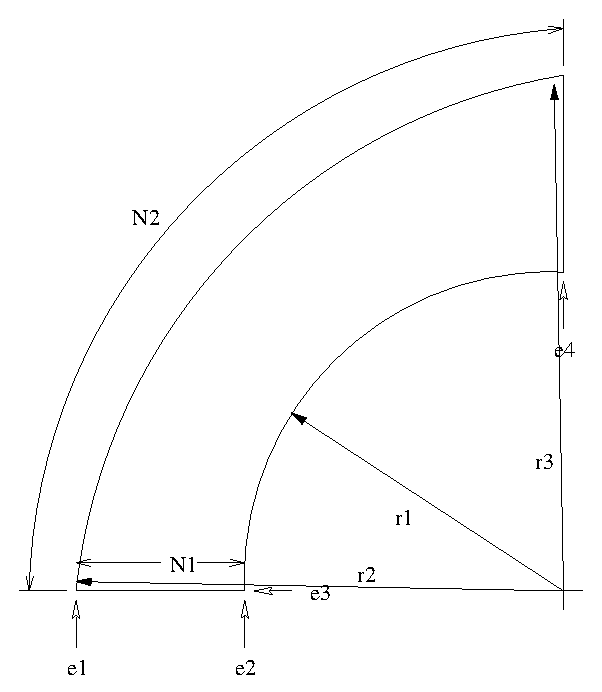
\includegraphics[width=3.0in]{gridBlunt2D.eps}
\caption{GridBlunt2D: constructing a 2D blunt body}
\label{fig:gridBlunt2D}
\end{figure}
%


%
\begin{figure}[h]
\vspace{0.3cm}
   \fontxfig
   \psfrag{e1}[][][1][0]{$\varepsilon_1$}
   \psfrag{e2}[bl][bl][1][0]{$\varepsilon_2$}
   \psfrag{t1}[r][r][1][0]{$\theta_1$}
   \psfrag{t2}[r][r][1][0]{$\theta_2$}
   \psfrag{L1}[t][t][1][0]{$L_1$}
   \psfrag{L2}[t][t][1][0]{$L_2$}
   \psfrag{L3}[br][br][1][0]{$L_3$}
   \psfrag{L4}[][][1][0]{$L_4$}
   \psfrag{L5}[t][t][1][0]{$L_5$}
   \psfrag{L6}[b][b][1][0]{$L_6$}
   \psfrag{L7}[b][b][1][0]{$L_7$}
   \psfrag{N1}[b][b][1][0]{$N_1$}
   \psfrag{N2}[b][b][1][0]{$N_2$}
   \psfrag{N3}[][][1][0]{$N_3$}
   \psfrag{N4}[][][1][0]{$N_4$}
   \psfrag{N5}[b][b][1][0]{$N_5$}
   \psfrag{N6}[t][t][1][0]{$N_6$}
   \psfrag{dz1}[b][b][1][0]{$\Delta \zeta_1$}
   \psfrag{dz2}[b][b][1][0]{$\Delta \zeta_2$}
   \psfrag{dz3}[bl][bl][1][0]{$\Delta \zeta_3$}
   \psfrag{dz4}[br][br][1][0]{$\Delta \zeta_4$}
   \psfrag{dz5}[b][b][1][0]{$\Delta \zeta_5$}
   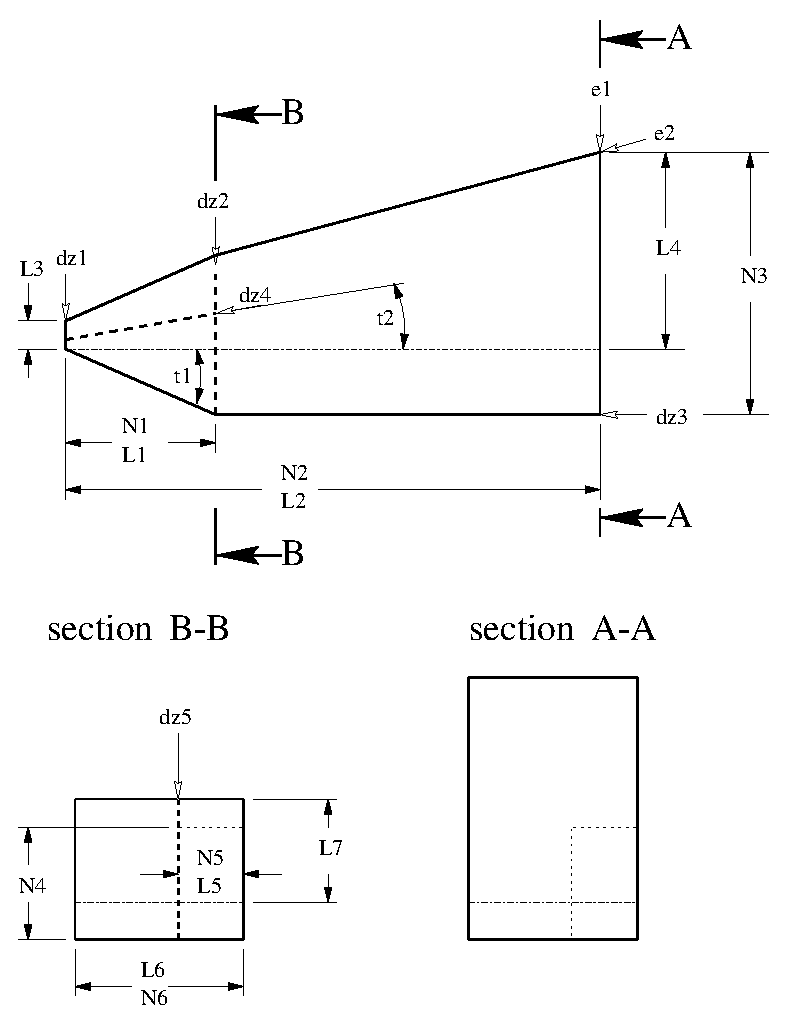
\includegraphics[width=6.0in]{gridRamp3D.eps}
\caption{GridRamp3D: constructing a 3D Ramp injector}
\label{fig:gridRamp3D}
\end{figure}
%

%
\begin{figure}[h]
\vspace{0.3cm}
   \fontxfig
   \psfrag{e1}[][][1][0]{$\varepsilon_1$}
   \psfrag{e2}[bl][bl][1][0]{$\varepsilon_2$}
   \psfrag{t1}[r][r][1][0]{$\theta_1$}
   \psfrag{t2}[r][r][1][0]{$\theta_2$}
   \psfrag{L1}[t][t][1][0]{$L_1$}
   \psfrag{L2}[t][t][1][0]{$L_2$}
   \psfrag{L3}[br][br][1][0]{$L_3$}
   \psfrag{L4}[][][1][0]{$L_4$}
   \psfrag{L5}[t][t][1][0]{$L_5$}
   \psfrag{L6}[b][b][1][0]{$L_6$}
   \psfrag{L7}[b][b][1][0]{$L_7$}
   \psfrag{L8}[b][b][1][0]{$L_8$}
   \psfrag{L9}[b][b][1][0]{$L_9$}
   \psfrag{L10}[b][b][1][0]{$L_{10}$}
   \psfrag{N1}[b][b][1][0]{$N_1$}
   \psfrag{N2}[b][b][1][0]{$N_2$}
   \psfrag{N3}[][][1][0]{$N_3$}
   \psfrag{N4}[][][1][0]{$N_4$}
   \psfrag{N5}[b][b][1][0]{$N_5$}
   \psfrag{N6}[t][t][1][0]{$N_6$}
   \psfrag{N7}[t][t][1][0]{$N_7$}
   \psfrag{N8}[t][t][1][0]{$N_8$}
   \psfrag{dz1}[b][b][1][0]{$\Delta \zeta_1$}
   \psfrag{dz2}[b][b][1][0]{$\Delta \zeta_2$}
   \psfrag{dz3}[bl][bl][1][0]{$\Delta \zeta_3$}
   \psfrag{dz4}[br][br][1][0]{$\Delta \zeta_4$}
   \psfrag{dz5}[b][b][1][0]{$\Delta \zeta_5$}
   \psfrag{dz6}[b][b][1][0]{$\Delta \zeta_6$}
   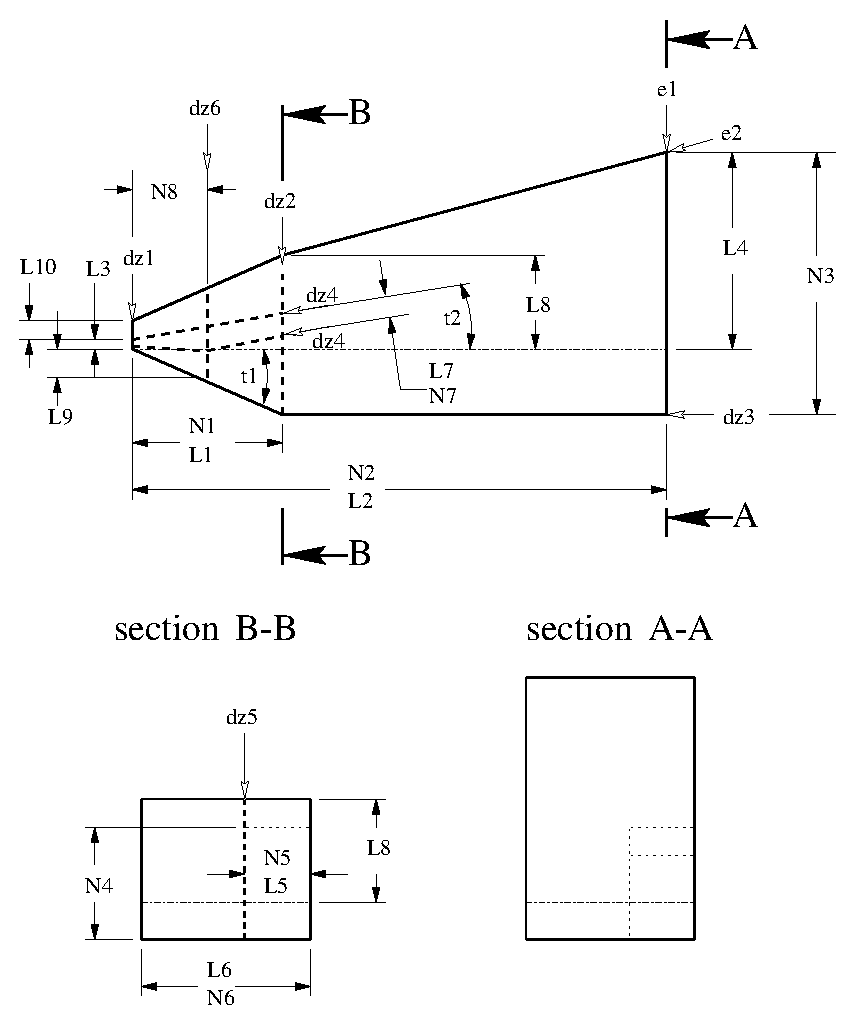
\includegraphics[width=6.0in]{gridCant3D.eps}
\caption{GridCant3D: constructing a 3D Cantilevered injector}
\label{fig:gridCant3D}
\end{figure}
%


%  \bibliographystyle{warpdoc}
%  \bibliography{all}


\end{document}













